\subsection{Veeltermfuncties of polynoomfuncties}
\label{sec:vtf}

\textbf{Functievoorschrift}

\begin{definitie}
	Een veelterm- of polynoomfunctie heeft als functievoorschrift een veelterm in 1 onbekende, dus
$f(x)=a_{n}x^{n}+a_{n-1}x^{n-1}+\ldots+a_{2}x^{2}+a_{1}x+a_{0}$
met $a_{n}\in\mathbb{R}_{0}$ en $a_{n-1},\ldots,a_{0}\in\mathbb{R}$. De constanten $a_{i}$ noemen we de \textbf{co\"effici\"enten}.

\end{definitie}

De (meestal eerste) term met de hoogste macht bepaalt de \textbf{graad} van de veeltermfunctie.

\begin{voorbeeld}
	$f(x)=2x^{4}-5x^{3}+10x$ , $f(x)=x^{3}$ 
\end{voorbeeld}

\textbf{Grafische voorstelling}

Het domein van een veeltermfunctie is: $\textrm{dom}f=\mathbb{R}$

De grafieken van de elementaire machtsfuncties $y=x^{n}$
met positieve exponent zijn hieronder weergegeven:
%TODO figuur vervangen
\gewonefiguur{height=5cm}{2_elem_rekenvaardigheden_B/inputs/veeltermfuncties1.jpg}

%\begin{figure}[h]
%\centering{}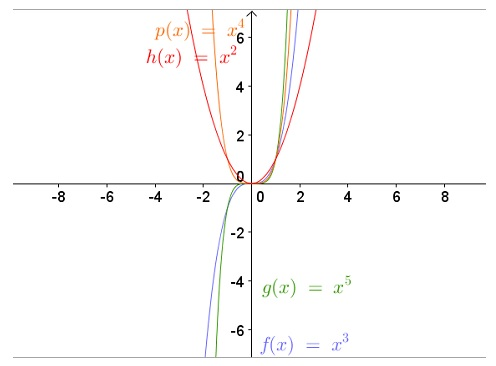
\includegraphics[height=5cm]{2_elem_rekenvaardigheden_B/inputs/veeltermfuncties1.jpg} 
%\end{figure}

De grafieken van de elementaire machtsfuncties $y=x^{-n}=\frac{1}{x^{n}}$
met negatieve exponent zijn hieronder weergegeven:

\gewonefiguur{height=5cm}{2_elem_rekenvaardigheden_B/inputs/veeltermfuncties2.jpg}

%\begin{figure}[h]
%\centering{}\includegraphics[height=5cm]{} 
%\end{figure}


\textbf{Nulwaarden}

 Een $n$\textsuperscript{de} graadsveeltermfunctie met oneven
$n$ heeft minimum $1$ en maximum $n$ snijpunten met de $x$-as.

 Een $n$\textsuperscript{de} graadsveeltermfunctie met even
$n$ heeft minimum $0$ en maximum $n$ snijpunten met de $x$-as. De grafiek
kan namelijk helemaal boven of onder de $x$-as liggen, en dus geen
snijpunten hebben met de $x$-as.



\begin{voorbeeld}
	De functie $f$ met voorschrift $f(x)=2x^{4}-3x^{3}-x^{2}+x$
is een 4\textsuperscript{de} graadsvergelijking en heeft in dit geval
4 snijpunten met de $x$-as:

\gewonefiguur{height=5cm}{2_elem_rekenvaardigheden_B/inputs/veeltermfuncties3.jpg}

%\begin{figure}[h]
%\centering{}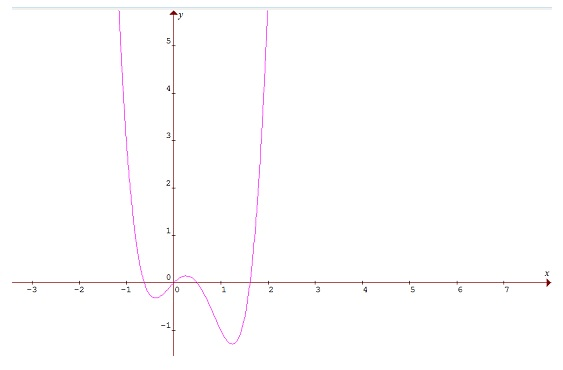
\includegraphics[height=5cm]{2_elem_rekenvaardigheden_B/inputs/veeltermfuncties3.jpg} 
%\caption{Voorbeeld veeltermfunctie.}
%\label{fig:vt:vb1}
%\end{figure}

\end{voorbeeld}

Nulwaarden vinden

De nulwaarden voor een veeltermfunctie vinden we door het
functievoorschrift te ontbinden in een product van factoren met ten
hoogste een tweede graad, m.a.w. we ontbinden de veeltermfunctie $f(x)$
in lineaire factoren $x+a$ en in kwadratische factoren $ax^{2}+bx+c$.
De nulpunten van de functie $f(x)$ zijn dan de nulpunten van de verschillende
factoren.

\textbf{Tekenverloop}

Eens een veelterm ontbonden is in factoren, is het eenvoudig
om het tekenverloop er van te bepalen. Het tekenverloop van een constante,
een lineaire en een kwadratische functie is immers gekend. Het teken
van een veeltermfunctie is het product van de tekens van de factoren.


\begin{voorbeeld}
	 (een tweedegraadsfunctie herleiden door substitutie)

Deze methode is toepasbaar bij bikwadratische vergelijkingen. Dit
zijn vergelijkingen van de vorm $ax^{4}+bx^{2}+c=0$. Dit type van
vergelijkingen kan herleid worden tot een kwadratische vergelijking
met behulp van de substitutiemethode. Stel hierbij $x^{2}=t$.

We bekijken de veelterm $f(x)=4x^{4}-5x^{2}+1$

Nulwaarden

 We bepalen de nulwaarden door de veelterm te ontbinden in
factoren, gebruik makend van de substitutiemethode:\\

\begin{equation*}
4x^{4}-5x^{2}+1=0 \ \   \underrightarrow{x^{2}=t}  \ \ 4t^{2}-5t+1=0
\end{equation*}

 We bekomen een kwadratische vergelijking. Hiervan zijn de
nulpunten:
\begin{eqnarray*}
t_{1}=\frac{-b+\sqrt{D}}{2a}&=&\frac{-(-5)+\sqrt{9}}{2.4}=1 \\
t_{2}=\frac{-b-\sqrt{D}}{2a}&=&\frac{-(-5)-\sqrt{9}}{2.4}=\frac{1}{4}
\end{eqnarray*}

De 2 oplossingen voor $t$ zijn $t_{1}=1$ en $t_{2}=\frac{1}{4}$
zodat de vergelijking kan geschreven worden als: $4t^{2}-5t+1=(t-1)(t-\frac{1}{4})$.

Aangezien $x^{2}=t$ zijn de 4 oplossingen voor $x$: $x_{1 \text{ en }2}=\pm\sqrt{t_{1}}$
en $x_{3 \text{ en } 4}=\pm\sqrt{t_{2}}$ 

Dit geeft $x_{1}=1$ , $x_{2}=-1$ , $x_{3}=\frac{1}{2}$
en $x_{4}=-\frac{1}{2}$.

De gegeven vergelijking kan dus ook geschreven worden als:

\begin{equation*}
f(x)=4x^{4}-5x^{2}+1=(x-1)(x+1)(x-\frac{1}{2})(x+\frac{1}{2})
\end{equation*}

Tekenverloop

Maak \'e\'en overzichtelijke tabel met bovenaan alle nulpunten
in stijgende volgorde. Per rij onderzoek je het teken van elke factor
van $f(x)$. Het teken van $f(x)$ is dan het product van deze tekens.

\begin{center}
\begin{tabular}{c||ccccccccc}
$x$ &  & $-1$ &  & $-\frac{1}{2}$ &  & $\frac{1}{2}$ &  & $1$ & \\
\hline 
$(x-1)$ & - & - & - & - & - & - & - & $0$ & $+$\\
$(x-\frac{1}{2})$ & - & - & - & - & -  & $0$ & + & + & + \\
$(x+\frac{1}{2})$ & - & - & - & $0$ & + & + & + & + & + \\
$(x+1)$ & $-$ & $0$ & + & + & + & + & + & + & + \\
\hline 
$f(x)$ & $+$ & $0$ & $-$ & $0$ & $+$ & $0$ & $-$ & $0$ & $+$\\
\end{tabular}
\end{center}

\end{voorbeeld}

\begin{voorbeeld}
	(ontbinden in factoren)

We bekijken de veelterm $f(x)=3x^{3}-4x^{2}-6x+8$

Nulwaarden

We bepalen de nulwaarden door de veelterm te ontbinden in
factoren. Soms kunnen we gebruik maken van merkwaardige producten
of, zoals in dit geval, door het groeperen van gemeenschappelijke
termen:

\begin{eqnarray*}
3x^{3}-4x^{2}-6x+8 & = & (3x^{3}-4x^{2})-(6x-8)\\
 & = & x^{2}(3x-4)-2(3x-4)\\
 & = & (x^{2}-2)(3x-4)\\
 & = & (x-\sqrt{2})(x+\sqrt{2})(3x-4)
\end{eqnarray*}

 De gegeven vergelijking $3x^{3}-4x^{2}-6x+8=0$ heeft dus
3 nulpunten:

\begin{equation*}
x_{1}=\sqrt{2}, x_{2}=-\sqrt{2} \text{ en } x_{3}=\frac{4}{3}
\end{equation*}

Tekenverloop

%Maak \'e\'en overzichtelijke tabel met bovenaan alle nulpunten
in stijgende volgorde. Per rij onderzoek je het teken van elke factor
van $f(x)$. Het teken van $f(x)$ is dan het product van deze tekens.

\begin{center}
\begin{tabular}{c||ccccccc}
$x$ &  & $-\sqrt{2}$ &  & $\frac{4}{3}$ &  & $\sqrt{2}$ & \\
\hline 
$(x-\sqrt{2})$ & - & - & -& -& - & $0$ & $+$ \\
$(x+\sqrt{2})$ & $-$ & $0$ & + & + & +&+&+ \\
$(3x-4)$ & - & - & - & $0$ & +&+&+ \\
\hline 
$f(x)$ & $-$ & $0$ & $+$ & $0$ & $-$ & $0$ & + \\
\end{tabular}
\end{center}


\end{voorbeeld}

\begin{voorbeeld}
	 (regel van Horner)

We bekijken de veelterm $f(x)=x^{4}-4x^{3}+5x^{2}-4x+4$

Nulpunten

We bepalen de nulpunten door de veelterm te ontbinden in
factoren gebruik makend van de regel van Horner.

Ga na welke mogelijke delers van $a_{0}$ kunnen afgesplitst
worden zonder rest. Hier zijn de delers van $a_{0}=4$: $\pm1,\:\pm2\:\textrm{en}\:\pm4$

We proberen $x=+2$: $f(2)=(2)^{4}-4(2)^{3}+5(2)^{2}-4(2)+4=0$

Dus de factor $(x-2)$ kan afgesplitst worden. De co\"effici\"enten
van de resterende veelterm vinden we via de regel van Horner:

\begin{center}
\begin{tabular}{r|rrrrr}
	& $1$ & $-4$ & $5$ & $-4$ & $4$\\
	$\mathbf{2}$ & $\downarrow$ & $2$ & $-4$ & $2$ & $-4$\\
	\hline  
	& $1$ & $-2$ & $1$ & \multicolumn{1}{r||}{$-2$} & $\mathbf{0}$\\
\end{tabular}	
\end{center}

We vinden $f(x)=x^{4}-4x^{3}+5x^{2}-4x+4=(x-2)(x^{3}-2x^{2}+x-2)$

We kunnen proberen om nog een factor af te splitsten.

We proberen nog eens $x=+2$: $f(2)=(2)^{3}-2(2)^{2}+(2)-2=0$

Dus de factor $(x-2)$ kan nog eens afgesplitst worden.
De co\"effici\"enten van de resterende veelterm vinden we terug via de
regel van Horner:

\begin{center}
\begin{tabular}{r|rrrr}
	& $1$ & $-2$ & $1$ & $-2$\\
	$\mathbf{2}$ & $\downarrow$ & $2$ & $0$ & $2$\\
	\hline 
	& $1$ & $0$ & \multicolumn{1}{r||}{$1$} & $\mathbf{0}$\\
\end{tabular}
\end{center}

We vinden tenslotte: $f(x)=x^{4}-4x^{3}+5x^{2}-4x+4=(x-2)^{2}(x^{2}+1)$

Merk op dat de discriminant $D$ van $(x^{2}+1)$ negatief
is zodat deze factor geen nulpunten heeft.

We vinden voor $x=2$ een dubbel nulpunt; deze veelterm
heeft dus 2 samenvallende snijpunten met de $x$-as.

Aangezien zowel de factor $(x-2)^{2}$ als ook de factor
$(x^{2}+1)$ steeds positief zijn, is er voor geen enkele waarde van
$x$ een negatief beeld (de functie bevindt zich overal boven de $x$-as,
en in het punt $x=2$ raakt deze veelterm de $x$-as).

\gewonefiguur{width=.6\linewidth}{2_elem_rekenvaardigheden_B/inputs/veeltermfuncties4.jpg}

Tekenverloop

Maak \'e\'en overzichtelijke tabel met bovenaan alle nulpunten
in stijgende volgorde. Per rij onderzoek je het teken van elke factor
van $f(x)$. Het teken van $f(x)$ is dan het product van deze tekens.

\begin{center}
\begin{tabular}{c||ccc}
$x$ &  & $2$ & \\
\hline 
$(x-2)^{2}$ & $+$ & $0$ & \multicolumn{1}{c}{$+$}\\
$(x^{2}+1)$ & +&+&+\\
\hline 
$f(x)$ & $+$ & $0$ & $+$\\
\end{tabular}
\par\end{center}

\end{voorbeeld}